\documentclass[a4paper,11pt,twoside]{article}
\usepackage[utf8]{inputenc}	%% Text coding
\usepackage[czech]{babel}
\usepackage{epsfig,subfigure}
\usepackage{amsfonts,amsmath,amssymb}
\usepackage{graphicx}
\usepackage[unicode]{hyperref}
\usepackage{indentfirst}
\usepackage{fancyhdr}
\usepackage{xifthen}
\usepackage{amsthm,thmtools}
\usepackage{bold-extra}
\usepackage[dvipsnames]{xcolor}

\hypersetup{
	pdftitle={Využití počítačů ve fyzice},
	pdfauthor={Pavel Stránský},
	pdffitwindow=true,
	colorlinks=true,
	urlcolor=cyan,            %barva textu pri tisku
	linkcolor=red,
	citecolor=green,
	filecolor=magenta
}

% Velikost stránky
\addtolength{\topmargin}{-1.5cm} %\addtolength{\textheight}{-10cm}
\addtolength{\textwidth}{4cm} \addtolength{\textheight}{4cm} % Šířka a výška textu
\addtolength{\voffset}{-0.5cm} % Horní okraj
\addtolength{\hoffset}{-2cm}
\setlength{\headheight}{15pt}

\pagestyle{fancy}

\DeclareMathOperator{\e}{e}

\def\vector#1{\boldsymbol{#1}}								% Vector
\renewcommand{\d}{\mathrm{d}}
\newcommand{\derivative}[3][]{\ifthenelse{\isempty{#1}}	    % Normal derivative
	{\frac{\d{#2}}{\d{#3}}}
	{\frac{\d^{#1}{#2}}{\d{#3}^{#1}}}
}
\def\makematrix#1{\begin{pmatrix}#1\end{pmatrix}}       % Matrix
\def\abs#1{\left|#1\right|}

\def\code#1{\textnormal{\texttt{#1}}}
\def\file#1{\textnormal{\textbf{\texttt{#1}}}}
\long\def\python#1{{\color{ForestGreen}#1}}

\newtheoremstyle{spaced}
{5pt}{5pt}{\itshape}{}{\bfseries}{:}{.5em}{}

\newtheoremstyle{red}
{5pt}{5pt}{\itshape\color{red}}{}{\bfseries\color{red}}{:}{.5em}{}

\newtheoremstyle{blue}
{5pt}{5pt}{\itshape\color{blue}}{}{\bfseries\color{blue}}{:}{.5em}{}

\begin{document}
\theoremstyle{spaced}
\newtheorem{example}{Příklad}[section]

\theoremstyle{red}
\newtheorem{task}{Úkol}[section]

\theoremstyle{blue}
\newtheorem{solution}{Řešení}[section]

\title{Zápisky k předmětu Využití počítačů ve fyzice}
\date{\today}
\author{Pavel Stránský}

\maketitle
\tableofcontents

\section{Obyčejné diferenciální rovnice}
    Každou obyčejnou diferenciální rovnici $n$-tého řádu lineární v nejvyšší derivaci lze převést na~soustavu $n$ obyčejných diferenciálních rovnic prvního řádu ve tvaru
    \begin{equation}\label{eq:ODR}
        \derivative{\vector{x}}{t}=\vector{f}(\vector{x},t),
    \end{equation}
    kde $\vector{x}=\vector{x}(t)$ je vektor hledaných funkcí.

\begin{example}
    Pohybovou rovnici
    \begin{equation}
        Ma=F(y),
    \end{equation}
    kde $M$ je hmotnost pohybujícího se tělesa, $y=y(t)$ jeho poloha a $a=a(t)=\d^{2}y/\d t^{2}$ převedeme na~dvě diferenciální rovnice prvního řádu triviálním zavedením rychlosti $v=v(t)=\d y/\d t$:
    \begin{equation}
        \derivative{}{t}\makematrix{y \\ v}=\makematrix{v \\ \frac{1}{M}F(y)},
    \end{equation}
    tj. vektor funkce pravých stran podle rovnice~\eqref{eq:ODR} je
    \begin{equation}
        \vector{f}(\vector{x},t)=\makematrix{v \\ \frac{1}{M}F(y)}
    \end{equation}
    kde $\vector{x}\equiv(y,v)$.
\end{example}

\begin{example}
    Pohybová rovnice pro harmonický oscilátor (matematické kyvadlo s malou výchylkou) při volbě jednotek $M=\Omega=1$, kde $M$ je hmotnost kmitající částice a $\Omega$ její rychlost, zní
    \begin{align}
        a&=\derivative[2]{y}{t}=-y &&\Longleftrightarrow &
        \derivative{}{t}\makematrix{y \\ v}&=\makematrix{v \\ t}
    \end{align}

\end{example}

\begin{task}
    Převeďte na soustavu obyčejných diferenciálních rovnic prvního řádu rovnici třetího řádu pro Hiemenzův tok
    \begin{equation}
        y'''+yy''-y'^{2}+1=0.
    \end{equation}
\end{task}

\begin{solution}
    Hledaná soustava diferenciálních rovnic je
    \begin{equation}
        \derivative{}{t}\makematrix{y \\ v \\ a}=\makematrix{v \\ a \\ -ya+v^{2}-1}.
    \end{equation}
\end{solution}

\subsection{Diferenciální rovnice prvního řádu}
    Drtivá většina knihoven a algoritmů pro integraci diferenciálních rovnic počítá s rovnicemi ve~tvaru~\eqref{eq:ODR}.
    Zde se omezíme na jednu rovnici
    \begin{equation}
        \derivative{y}{t}=f(y,t),
    \end{equation}
    přičemž rozšíření na soustavu je triviální: místo skalárů $y$ a $f$ vezmeme vektory.

    Řešení diferenciální rovnice spočívá v nahrazení infinitezimálních přírůstků přírůstky konečnými:
    \begin{equation}\label{eq:Difference}
        \frac{\Delta y}{\Delta t}=\phi(y,t)
    \end{equation}
    kde $\phi$ je funkce, která udává směr, podél kterého se při numerickém řešení vydáme.
    Volbá této funkce je klíčová a záleží na ní, jak přesné řešení dostaneme a jak rychle ho dostaneme.

    \subsubsection{Pár důležitých pojmů}
    \begin{itemize}
        \item {\bf Jednokrokové algoritmy:}
        Algoritmy, které výpočtu následujícího kroku hodnoty funkce $y_{i+1}$ vyžadují znalost pouze aktuálního kroku $y_{i}$.
        Rozepsáním~\eqref{eq:Difference} dostaneme
        \begin{equation}
            \boxed{
                y_{i+1}=y_{i}+\underbrace{\phi(y_{i},t)}_{\phi_{i}}\Delta t
            },
        \end{equation}
        přičemž počáteční hodnota $y_{0}$ je dána počáteční podmínkou.
        My se omezíme pouze na tyto algoritmy.

        \item {\bf Lokální diskretizační chyba:}
        \begin{equation}
            \mathcal{L}=y(t+\Delta t)-y(t)-\phi(y(t),t)\Delta t,
        \end{equation}        
        kde $y(t)$ udává přesné řešení v čase $t$.

        \item {\bf Akumulovaná diskretizační chyba:}
        \begin{equation}
            \epsilon_{i}=y_{i}-y(t_{i})
        \end{equation}

        \item {\bf Řád metody:} 
        Metoda je $p$-tého řádu, pokud
        \begin{equation}\label{eq:MethodOrder}
            L(\Delta t)=\mathcal{O}(\Delta t^{p+1}).
        \end{equation}

        \item {\bf Symplektické algoritmy:}
        Speciální algoritmy navržené pro řešení pohybových di\-fe\-ren\-ci\-ál\-ních rovnic.
        Od běžných algoritmů je odlišuje to, že zachovávají objem fázového prostoru, a~tedy i energii (zatímco u obecných algoritmů se energie s integračním časem mění a většinou roste).
        V praxi se ze~symplektických algoritmů používá pouze Verletův algoritmus~\ref{sec:Verlet}.

        \item {\bf Kontrola chyby řešení:}
        Chybu numerického řešení diferenciální rovnice lze zmenšit 1)~men\-ším krokem, 2)~lepší metodou (metodou vyššího řádu). 
        Menší krok však znamená vyšší vý\-po\-čet\-ní čas.
        Sofistikované metody proto průběžně mění velikost kroku: když se funkce mění pomalu, krok prodlouží, když se mění rychle, krok zkrátí (tzv. {\bf metody s adaptivním krokem}).
        Tím se docílí vysoké přesnosti při co nejmenším výpočetním čase.

    \end{itemize}

    \subsubsection{Eulerova metoda 1. řádu}
        \begin{equation}\label{eq:Euler1}
            \phi_{i}=f(y_{i},t_{i}),
        \end{equation}
        tj. krok do $y_{i+1}$ děláme vždy ve směru tečny v bodě $y_{i}$.

        \begin{itemize}
            \item Nejjednodušší metoda integrace diferenciálních rovnic.
            \item Chyba je obrovská, k dosažení přesných hodnot je potřeba velmi malého kroku, což znamená dlouhý výpočetní čas.
        \end{itemize}

    \subsubsection{Eulerova metoda 2. řádu}
        \begin{align}\label{eq:Euler2a}
            k_{1}&=f(y_{i},t_{i})\nonumber\\
            k_{2}&=f\left(y_{i}+k_{1}\Delta t,t+\Delta t\right)\\
            \phi_{i}&=\frac{1}{2}\left(k_{1}+k_{2}\right),\nonumber
        \end{align}
        tj. uděláme jednoduchý Eulerův krok ve směru $k_{1}$, spočítáme derivaci $k_{2}$ po tomto kroku a vyrazíme z bodu $y_{i}$ ve směru, který je průměrem obou směrů (doporučuji si nakreslit obrázek).

        Ekvivalentní je udělat \uv{Eulerův půlkrok} a vyrazit z bodu $y_{i}$ ve směru derivace spočtené po~tomto půlkroku:
        \begin{align}\label{eq:Euler2b}
            k'_{1}&=f(y_{i},t_{i})\nonumber\\
            k'_{2}&=f\left(y_{i}+k'_{1}\frac{\Delta t}{2},t+\frac{\Delta t}{2}\right)\\
            \phi_{i}&=k'_{2}\nonumber
        \end{align}

    \subsection{Runge-Kuttova metoda 4. řádu}
        \begin{align}\label{eq:RungeKutta}
            k_{1}&=f(y_{i},t_{i})\nonumber\\
            k_{2}&=f\left(y_{i}+k_{1}\frac{\Delta t}{2},t+\frac{\Delta t}{2}\right)\nonumber\\
            k_{3}&=f\left(y_{i}+k_{2}\frac{\Delta t}{2},t+\frac{\Delta t}{2}\right)\\
            k_{4}&=f\left(y_{i}+k_{3}\Delta t,t+\Delta t\right)\nonumber\\
            \phi_{i}&=\frac{1}{6}\left(k_{1}+2k_{2}+2k_{3}+k_{4}\right)\nonumber
        \end{align}
        
        \begin{itemize}
            \item Jedna z nejčastěji používaných metod.
            \item Vysoká rychlost a přesnost při relativní jednoduchosti.
            \item Existují i Runge-Kuttovy metody vyššího řádu $p$, avšak vyžadují výpočet více než $p$ dílčích derivací $k_{j}$.
            Obecně platí, že metoda řádu $p\leq4$ vyžaduje $p$ derivací, metoda řádu $5\leq p\leq7$ vyžaduje $p+1$ derivací a metoda řádu $p=8,9$ vyřaduje $p+2$ derivací.
        \end{itemize}

    \subsection{Verletova metoda}\label{sec:Verlet}
        Pro rovnici 2. řádu ve tvaru (pohybovou rovnici)
        \begin{equation}\label{eq:EM}
            M\derivative[2]{y}{t}=F(y),
        \end{equation}
        kde $M$ je hmotnost pohybující se částice a $F$ síla, která na ni působí.
        Algoritmus je
        \begin{align}
            y_{i+1}&=y_{i}+v_{i}\Delta t+\frac{1}{2}a_{i}\Delta t^{2},\nonumber\\
            v_{i+1}&=v_{i}+\frac{1}{2}\left(a_{i+1}+a_{i}\right)\Delta t,
        \end{align}
        kde $a_{i}\equiv F(y_{i})/M$.

        \begin{itemize}
            \item Symplektický algoritmus, tj. algoritmus zachovávající energii (pokud systém popsaný rovnicí~\eqref{eq:EM} energii zachovává).
            \item Užívá se nejčastěji v molekulární dynamice k simulaci pohybu velkého množství vzájemně interagujících částic.
            \item Řád této metody je $p=2$. Symplektické algoritmy s vyšším řádem existují, avšak v praxi se nepoužívají.
        \end{itemize}

    \begin{task}
        Naprogramujte Eulerovu metodu 1. a 2. řádu\footnote{Tyto metody jsme již naprogramovali na cvičení minulý týden.}, Runge-Kuttovu metodu a Verletovu metodu a vyřešte diferenciální rovnici harmonického oscilátoru
        \begin{equation}\label{eq:HO}
            \derivative[2]{y}{t}=-y
        \end{equation}
        s počátečními podmínkami $y_{0}=0$, $y'_{0}\equiv v_{0}=1$ (analytickým řešením je funkce $\sin t$).
        Časový krok ponechte jako volný parametr.
        Nakreslete grafy řešení $y(t)$ a grafy energie $E(t)$ pro rozdílné hodnoty integračních kroků, například $\Delta t=0.01$ a $\Delta t=0.1$ pro čas $t\in\langle0;30\rangle$.
        Energie harmonického oscilátoru je dána vzorcem
        \begin{equation}\label{eq:HOE}
            E=\frac{1}{2}\left(y^{2}+v^{2}\right).
        \end{equation}
        Přesvědčte se, že jediná Verletova metoda skutečně zachovává energii. 
        Pro ostatní metody energie roste.
    \end{task}

    \begin{solution}
        Jedno možné řešení je rozděleno do dvou souborů \file{ODE.py} a \file{Oscillator.py}, které můžete stáhnout z GitHubu \textnormal{\url{https://www.github.com/PavelStransky/PCInPhysics}}  (o GitHubu bude pojednáno v sekci~\ref{sec:GITRemote}). 

        \begin{itemize}
        \item \file{ODE.py}: 
            Modul napsaný dostatečně obecně, aby ho bylo možné použít na řešení libovolných soustav diferenciálních rovnic.
            \begin{itemize}
            \item \code{StepEuler1}: 
                Integrační krok Eulerovy metody 1. řádu.
            \item \code{StepEuler2}: 
                Integrační krok Eulerovy metody 2. řádu.
            \item \code{StepVerlet}: 
                Integrační krok Verletovy metody.
            \item \code{StepRungeKutta}: 
                Integrační krok Runge-Kuttovy metody 4. řádu.
            \item \code{ODESolution}: 
                Integruje diferenciální rovnici danou pravými stranami prvního parametru \code{Derivatives} pomocí kroku (metody) dané parametrem \code{Step} a délkou \code{dt}, přičemž vrátí pole hodnot řešení soustavy rovnic v jednotlivých časech, pole časů a jméno integračního kroku (pro snazší pozdější porovnání různých metod).
            \item \code{ScipyODESolution}: 
                Integruje diferenciální rovnici pomocí funkce \code{odeint} z knihovny \code{scipy.integrate}. 
                Pozor, parametr \code{dt} zde neznamená integrační krok, nýbrž časový krok výsledného pole.
                Funkce \code{odeint} používá sofistikovaný řešitel diferenciálních rovnic s proměnným krokem.
                Pro podrobnosti můžete mrknout na \href{https://docs.scipy.org/doc/scipy/reference/generated/scipy.integrate.odeint.html}{dokumentaci} k této funkci.

            \item \code{ShowGraphSolutions}:
                Vykreslí graf řešení diferenciální rovnice (jako první parametr \code{odeSolutions} lze zadat seznam více řešení různými metodami či s různým krokem).
                Parametr \code{ExactFunction} je odkaz na přesné řešení dané diferenciální rovnice. 
                Je-li specifikován, vykreslí se do grafu dva panely: jeden s hodnotami numerického řešení, druhý s rozdílem řešení numerického a přesného.                 
            \end{itemize}
            Funkce \code{StepEuler1}, \code{StepEuler2} a \code{StepRungeKutta} fungují pro obecnou soustavu $n$ o\-by\-čej\-ných diferenciálních rovnic prvního řádu.
            Funkce \code{StepVerlet} funguje jen pro pohybovou rovnici, tj. pro jednu diferencální rovnici původně druhého řádu přepsanou na dvě diferenciální rovnice prvního řádu.

        \item \file{Oscillator.py}:
            Soubor, který využívá obecných funkcí z modulu \file{ODE.py} pro integraci harmonického oscilátoru různými metodami.
            \begin{itemize}
            \item \code{Energy}:
                Pro zadanou polohu a rychlost vrátí energii harmonického oscilátoru.
            \item \code{Derivatives}:
                Pravá strana soustavy diferenciálních rovnic harmonického oscilátoru. 
            \item \code{CompareMethods}:
                Vyřeší diferenciální rovnici harmonického oscilátoru různými metodami a řešení nakreslí do jednoho grafu.
                Následně vykreslí grafy $E(t)$.
                Harmonický oscilátor je konzervativní systém (zachovává energii), rostoucí energie je způsobena ne\-přes\-nos\-tí integrační metody.
            \end{itemize}
        \end{itemize}

        \begin{figure}[!htbp]
            \centering
			\subfigure{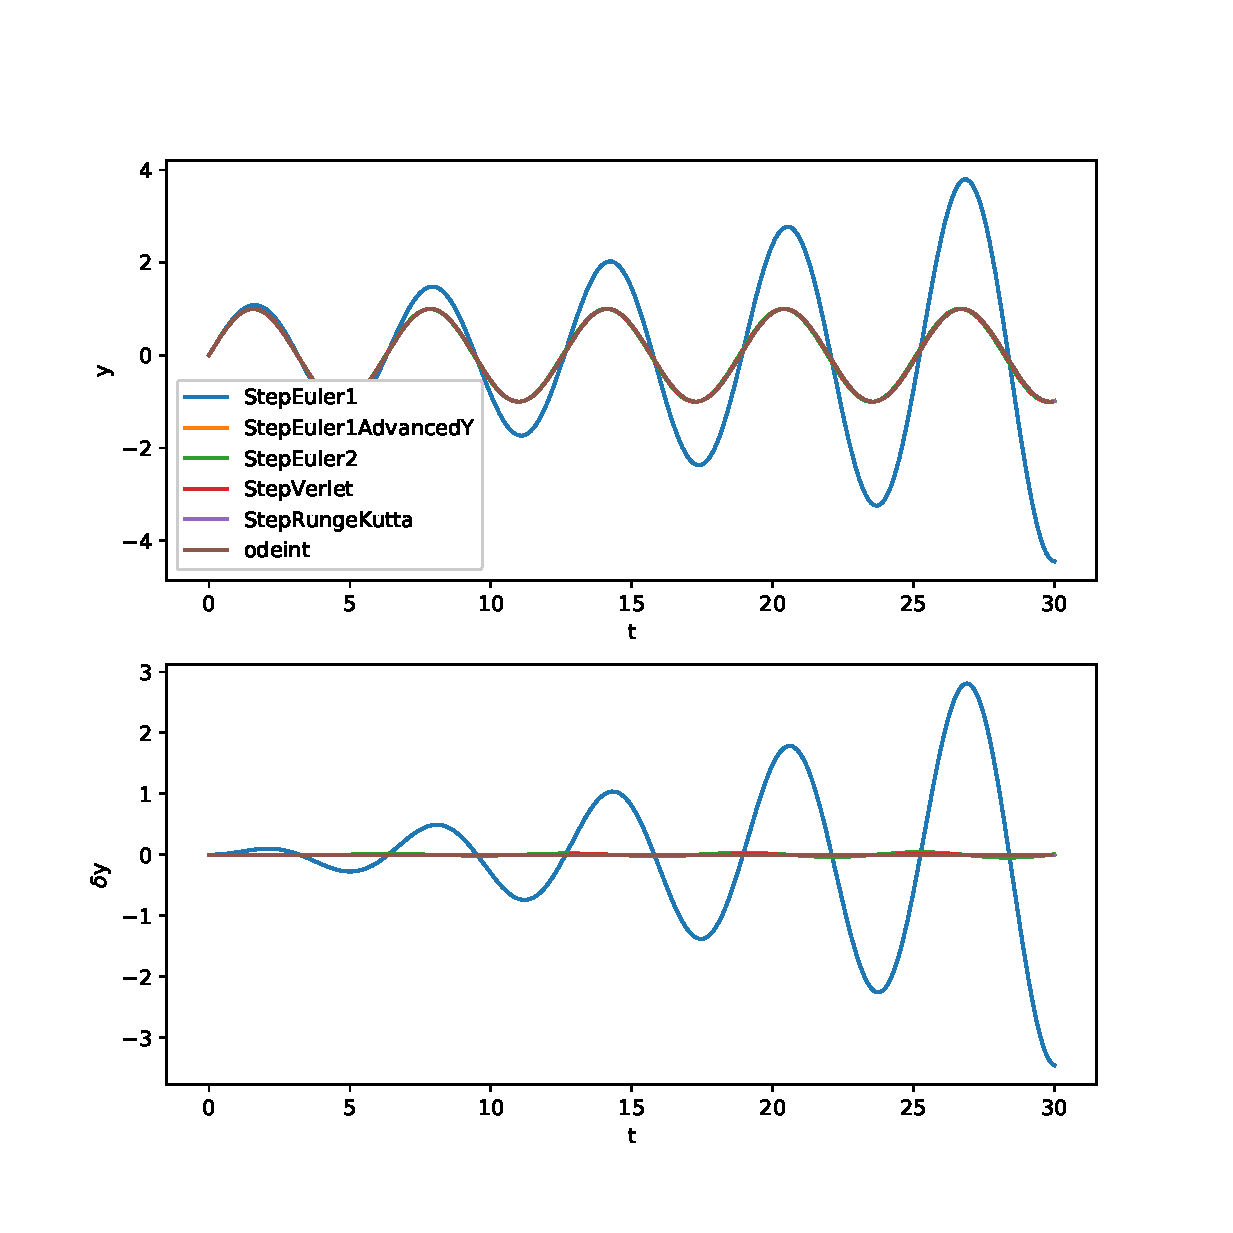
\epsfig{file=oscillator.eps,width=0.49\linewidth,keepaspectratio}}
			\subfigure{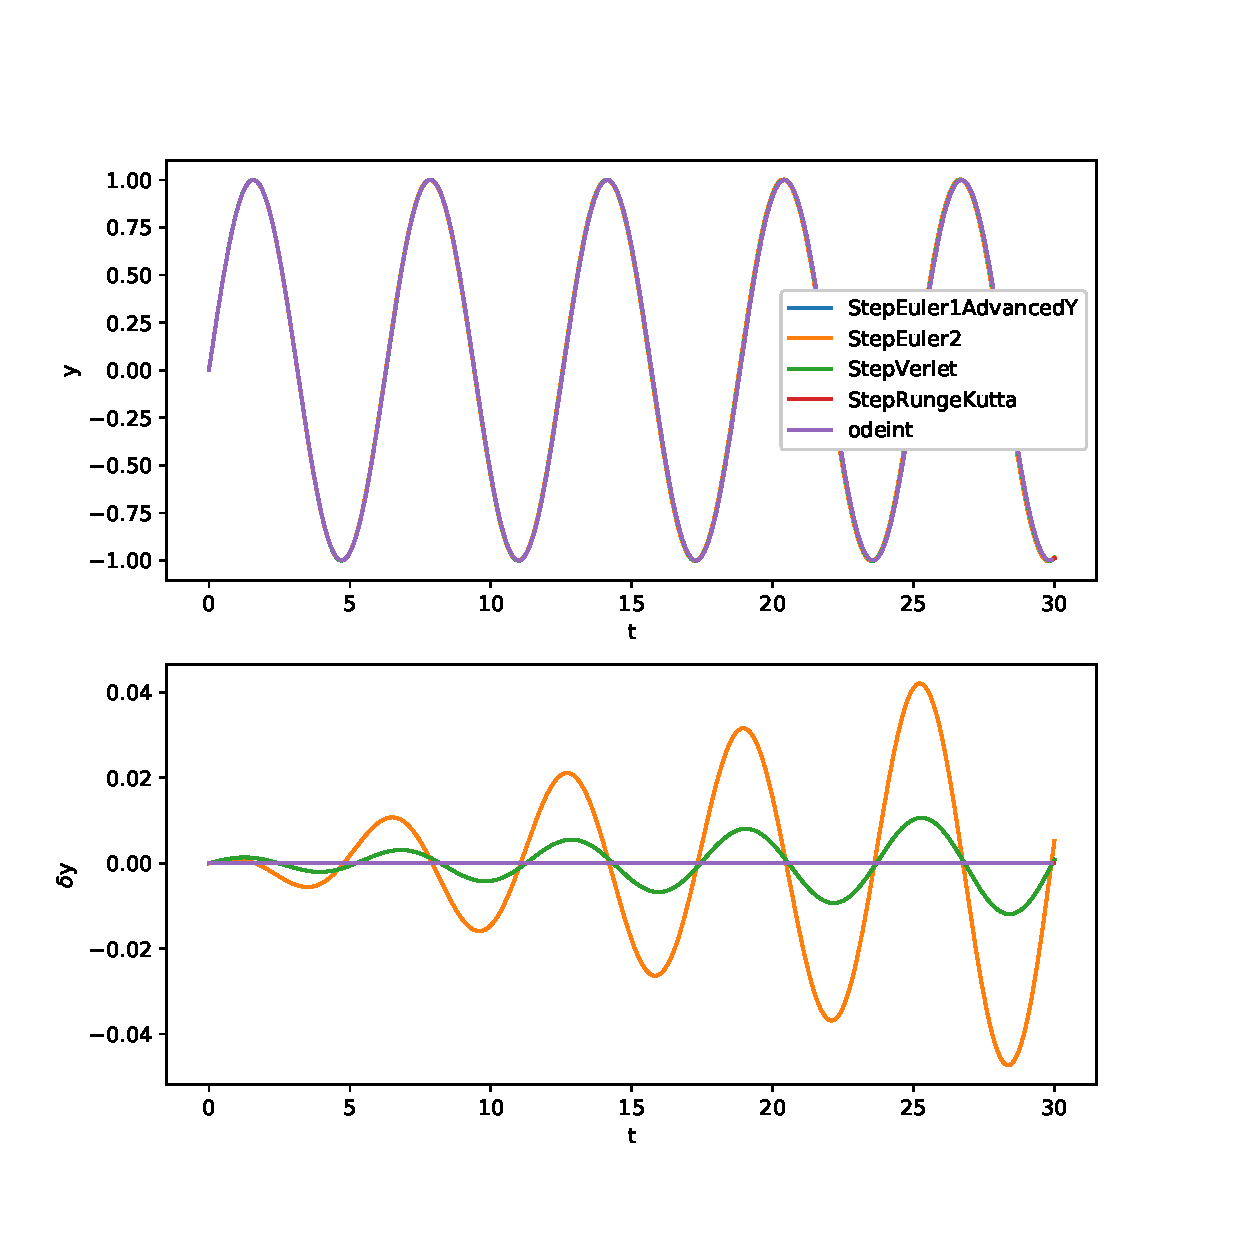
\epsfig{file=oscillator2.eps,width=0.49\linewidth,keepaspectratio}}\\
			\subfigure{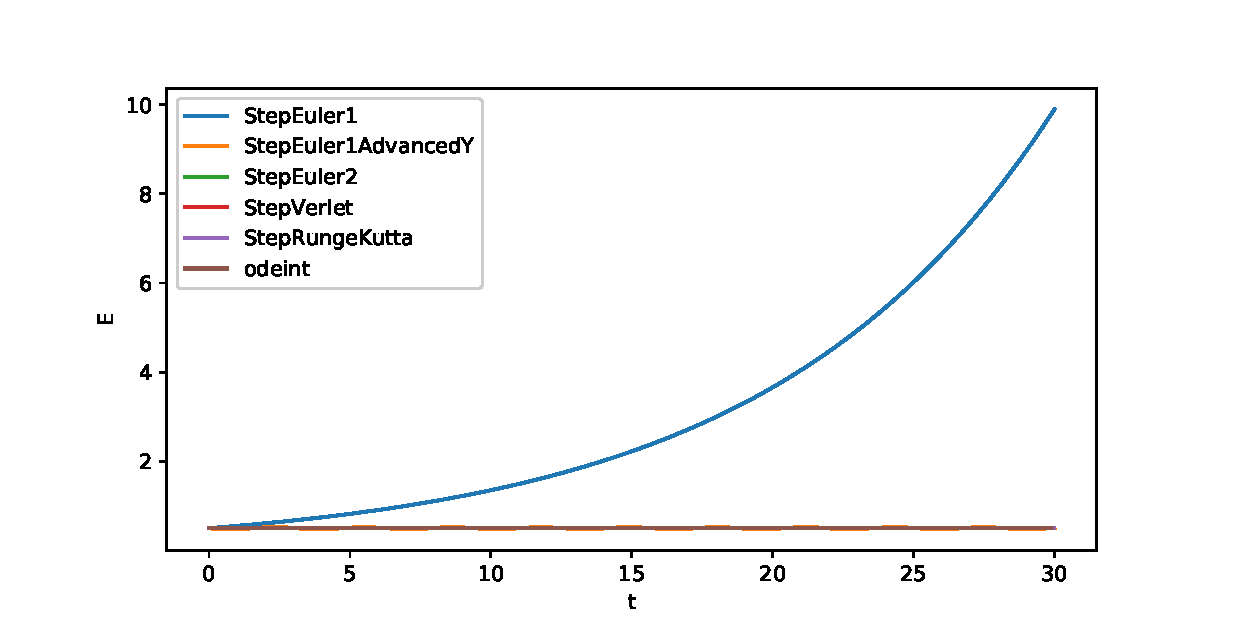
\epsfig{file=oscillator_energy.eps,width=0.49\linewidth,keepaspectratio}}
			\subfigure{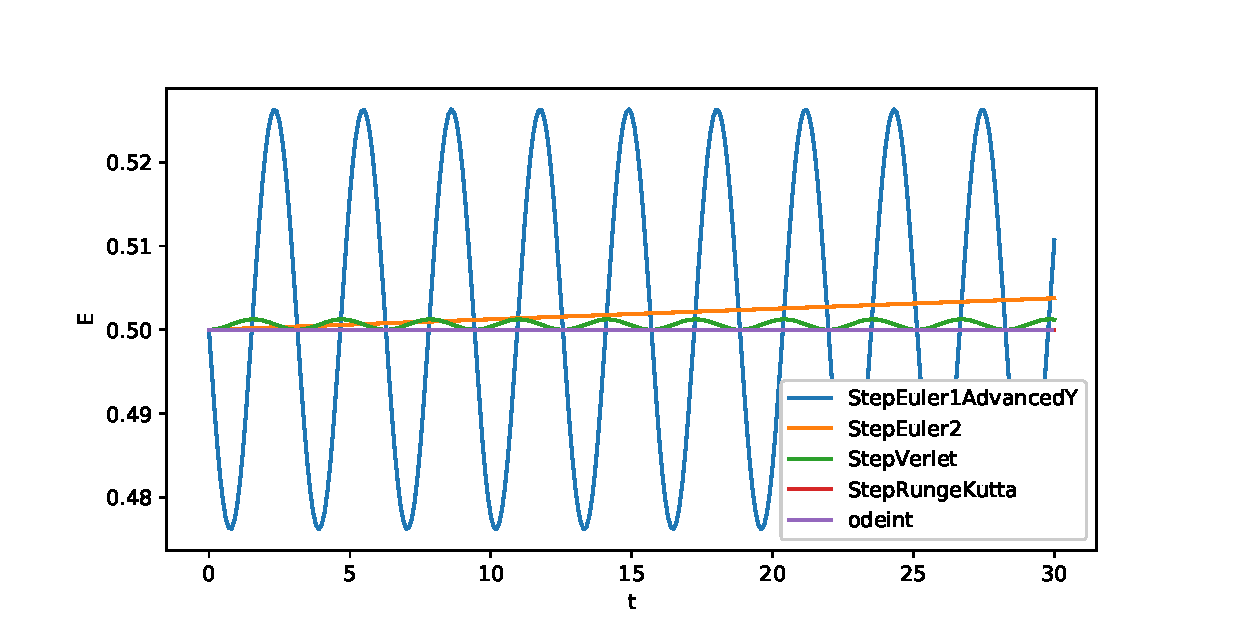
\epsfig{file=oscillator_energy2.eps,width=0.49\linewidth,keepaspectratio}}\\
			\caption{
                \protect\small
                Integrace diferenciální rovnice harmonického oscilátoru~\eqref{eq:HO} různými metodami.
                Časový krok je $\Delta t=0.1$.
                \emph{Levý sloupec:} všechny metody.
                \emph{Pravý sloupec:} bez Eulerovy metody 1. řádu.
                \emph{1.~řádek:} hodnoty $y(t)$.
                \emph{2.~řádek:} rozdíly $\delta y(t)=y(t)-\sin{t}$.
                Pro Eulerovu metodu 1. řádu je divergence numerického od analytického řešení očividně exponenciální v čase.
                \emph{3.~řádek:} energie~\eqref{eq:HOE}. 
                Pro Eulerovy metody energie roste.
                Energie se mění i pro Runge-Kuttovu metodu (pro tento systém energie s časem klesá) a pro integraci pomocí funkce \code{odeint}, avšak tyto změny jsou řádově menší, a tudíž je není na grafech při daném měřítku svislé osy vidět.
                Naopak pro Verletův algoritmus a pro \uv{předbíhající} Eulerovu metodu energie osciluje okolo počáteční energie $E=\frac{1}{2}$.
            }	
            \label{fig:HO}
		\end{figure}

        Příslušné grafy jsou zobrazeny v obrázku~\ref{fig:HO}.
    \end{solution}

    \begin{task}
        Rozšiřte kód tak, aby počítal průměrnou kumulovanou chybu
        \begin{equation}\label{eq:HOError}
            \mathcal{E}=\sqrt{\frac{1}{n}\sum_{i=0}^{n-1}\left(y_{i}-\sin t_{i}\right)^{2}}
        \end{equation}
        a nakreslete závislost $E(\Delta t)$ pro $\Delta t\in\langle0.002;0.1\rangle$ a pro různé metody.
        Jelikož očekáváme mocninnou závislost dle~\eqref{eq:MethodOrder}, kde exponent je tím větší, čím větší je řád metody, je výhodné graf $E(\Delta t)$ kreslit v log-log měřítku.
        V Pythonu použijete místo \textnormal{\texttt{plot(...)}} funkci \textnormal{\texttt{loglog(...)}} z knihovny \textnormal{\texttt{matplotlib.pyplot}}.
    \end{task}

    \begin{solution}
        Průměrnou kumulovanou chybu počítá funkce \code{CumulativeError} z modulu \file{ODE.py}.
        Srovnání řešení diferenciální rovnice harmonického oscilátoru různými integračními metodami zakresluje do grafu funkce \code{ShowGraphCumulativeErrors} ze souboru \file{Oscillator.py}.
        Výsledný graf je znázorněn na obrázku~\ref{fig:HOError}.
        Vypočítanými křivkami $\ln\mathcal{E}(\ln\Delta t)$ je proložena přímka, jejíž sklon $\alpha$ udává exponent moncinného zákona
        \begin{equation}
            \mathcal{E}\propto\left(\Delta t\right)^{\alpha}
        \end{equation} 
        (k proložení přímky je využita funkce pro lineární regresi \code{linregress} z knihovny \code{scipy.stats}).
        Tento exponent výborně odpovídá řádu metody $p$ dle rovnice~\eqref{eq:MethodOrder}.

        \begin{figure}[!htbp]
            \centering
			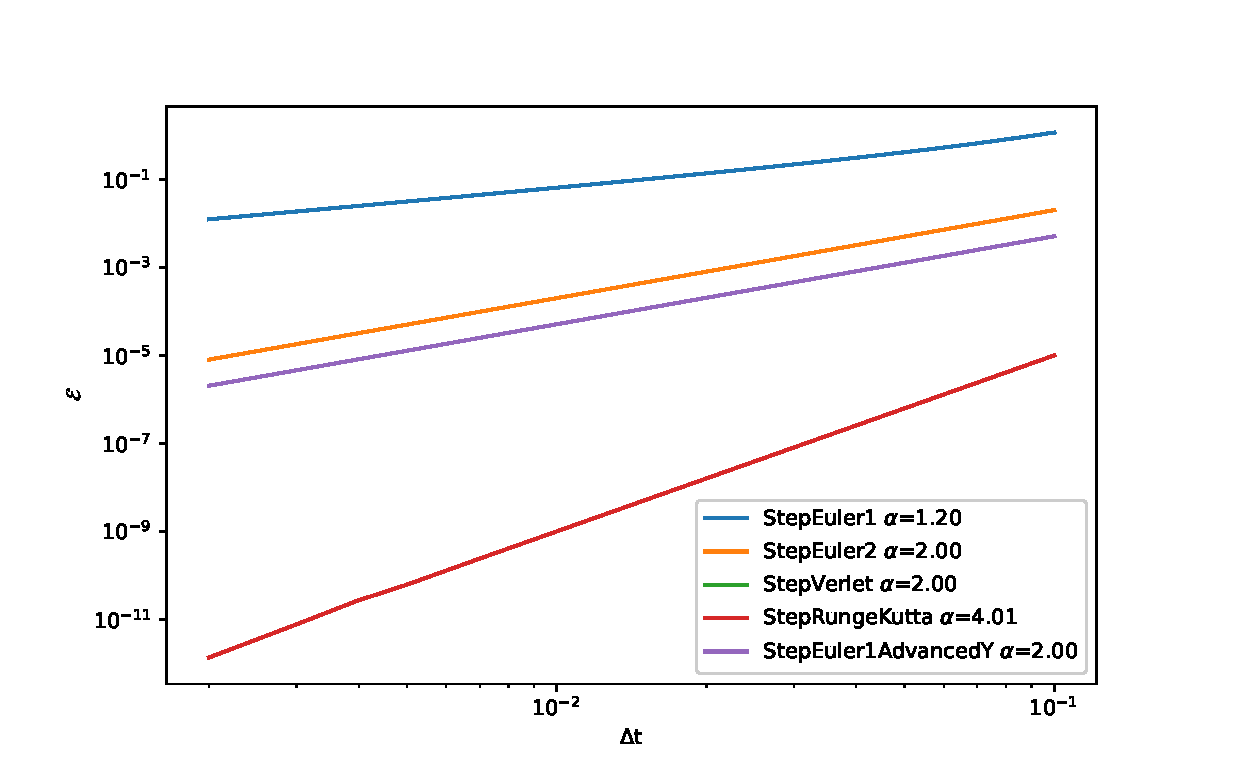
\epsfig{file=oscillator_error.eps,width=0.8\linewidth,keepaspectratio}
			\caption{
                \protect\small
                Závislost průměrné kumulované chyby~\eqref{eq:HOError} na délce kroku $\Delta t$ vypočítaná a vykreslená pomocí funkce \code{ShowGraphCumulativeErrors} pro harmonický oscilátor (soubor \file{Oscillator.py}).
                Křivka pro Verletovu metodu je \uv{schovaná} za křivkou pro předbíhající Eulerovu metodu.
            }	
            \label{fig:HOError}
		\end{figure}
    \end{solution}

    \begin{task}
        Eulerovu metodu 1. řádu lze pro harmonický oscilátor vylepšit následující záměnou:
        \begin{align}
            &\begin{matrix}
                y_{i+1}=y_{i}+v_{i}\Delta t \\
                v_{i+1}=v_{i}-y_{i}\Delta t 
            \end{matrix}
            &&\longrightarrow
            &\begin{matrix}
                y_{i+1}=y_{i}+v_{i}\Delta t \\
                v_{i+1}=v_{i}-y_{i+1}\Delta t 
            \end{matrix}
        \end{align}
        (vypočítáme $y_{i+1}$ a tuto hodnotu použijeme namísto hodnoty $y_{i}$ pro výpočet rychlosti $v_{i+1}$).
        Naprogramujte tuto metodu u ukažte, že pro harmonický oscilátor se jedná o metodu 2. řádu.
        Využijte srovnání v grafu z předchozí úlohy.
    \end{task}

    \begin{solution}
        Tato metoda je naimplementována v modulu \file{ODE.py} funkcemi \code{StepEuler1AdvancedY} a \code{StepEuler1AdvancedV}.
        Ze srovnání s ostatními metodami zobrazené v obrázcích~\ref{fig:HO} a~\ref{fig:HOError} vyplývá, že tato metoda je
        \begin{itemize}
        \item symplektická (energie sice osciluje a osciluje s větší amplitudou než pro Verletovu metodu, ale pořád osciluje okolo počáteční hodnoty),
        \item 2. řádu.
        \end{itemize}
        V obrázcích jsou výsledky pouze pro metodu předbíhající v souřadnici. 
        Díky symetrii jsou výsledky pro metodu předbíhající v rychlosti identické.
    \end{solution}

    \begin{task}
        Využijte hotové kódy a pohrajte si s řešením rovnice pro klesající exponenciálu
        \begin{equation}\label{eq:Exp}
            \derivative[2]{y}{t}=y
        \end{equation}
        s počátečními podmínkami $y_{0}=1$, $y'_{0}=-1$.
        Přesvědčte se, že Verletova metoda a vylepšená Eulerova metoda z posledního bodu jsou nestabilní --- pro tuto rovnici v relativně krátkém čase začnou řešení exponenciálně divergovat.
    \end{task}

    \begin{solution}
        Řešení analogické k příkladu harmonického oscilátoru je v souboru \file{Exp.py}.
        Tento systém není konzervativní --- nelze nadefinovat zachovávající se veličinu, která by měla význam energie.

        \begin{figure}[!htbp]
            \centering
			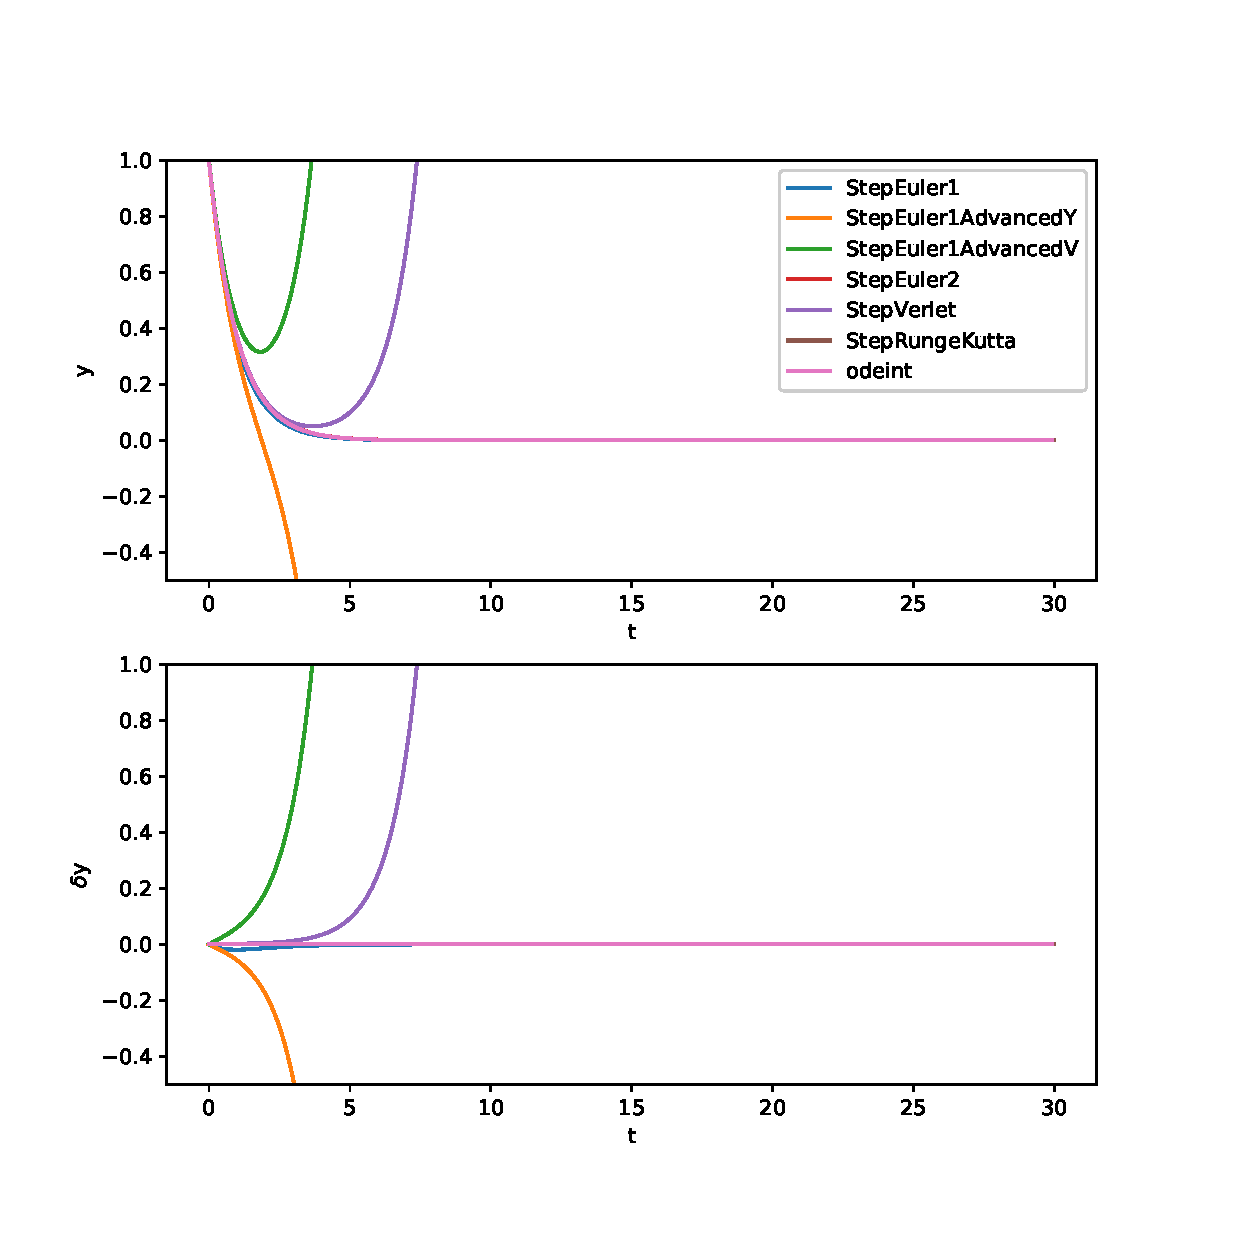
\epsfig{file=exp.eps,width=0.8\linewidth,keepaspectratio}
			\caption{
                \protect\small
                Totéž jako v obrázku~\ref{fig:HO}, avšak pro exponenciálně klesající systém daný rovnicí~\eqref{eq:Exp}.
                Symplektické algoritmy jsou nestabilní.
                }	
            \label{fig:Exp}
        \end{figure}
        
        \begin{figure}[!htbp]
            \centering
			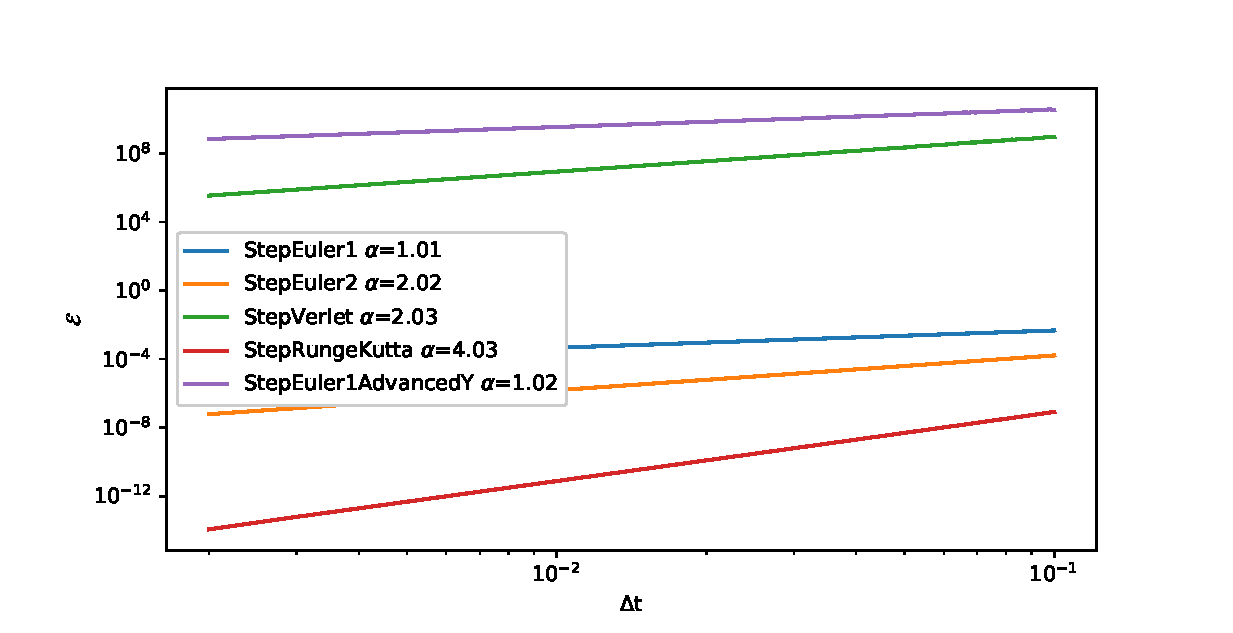
\epsfig{file=exp_error.eps,width=0.8\linewidth,keepaspectratio}
			\caption{
                \protect\small
                Totéž jako v obrázku~\ref{fig:HOError}, avšak pro exponenciálně klesající systém daný rovnicí~\eqref{eq:Exp}.
                Pro symplektické algoritmy uvedený graf nedává příliš smysl, jelikož chyba je o řády vyšší než hledané řešení.
                Přesto stojí za povšimnutí, že předbíhající Eulerův algoritmus, který výborně funguje pro harmonický oscilátor a je pro něj metodou 2. řádu, se zde chová jako metoda 1. řádu.
            }	
            \label{fig:ExpError}
        \end{figure}

        Z obrázku~\ref{fig:Exp} je vidět, že symplektické algoritmy jsou zde nestabilní, a tudíž nejsou na tento typ úlohy vhodné, což je pochopitelné, protože symplektické algoritmy jsou navrženy pouze pro energii zachovávající systémy.
        Obecné řešení rovnice~\eqref{eq:Exp} má tvar
        \begin{equation}
            y(t)=A\e^{t}+B\e^{-t},
        \end{equation}
        přičemž my speciálními počátečními podmínkami vybíráme pouze exponenciálně klesající řešení.
        Symplektické algoritmy v určitou chvíli \uv{překmitnou} na exponenciálně rostoucí řešení a začnou divergovat.

        Průměrná kumulovaná chyba je znázorněna na obrázku~\ref{fig:ExpError}. 
    \end{solution}

    \subsection{Shrnutí}
    \begin{itemize}
    \item 
        Řešitelé obyčejných diferenciálních rovnic převážně pracují se soustavami diferenciálních rovnic prvního řádu.
        Na tento tvar není obtížné diferenciální rovnici vyššího řádu převést.

    \item
        Nejčastěji se používají jednokrokové metody, jejichž hlavní výhoda je v možnosti jednoduše měnit délku kroku.

    \item 
        Přesnost řešení závisí na řádu metody $p$ a na délce integračního kroku $\Delta t$.
        Čím je řád metody vyšší, tím rychleji klesá chyba se zmenšujícícm se krokem.
        V praxi, pokud nechcete svěřit svůj probém černé skříňce ve formě nějaké hotové knihovny, se velmi často používá Runge-Kuttova metoda 4. řádu, která je jednoduchá na implementaci, je stabilní a rychlá.

    \item
        Symplektické metody, z nichž nejběžnější je Verletova metoda, jsou výhodné k modelování fyzikálních systémů zachovávajících energii.
        Pro nekonzervativní systémy nejsou vhodné. 

    \item
        \python{V Pythonu se procvičilo:
        \begin{itemize}
        \item
            předávání odkazů na funkce v argumentu,

        \item
            vracení více hodnot z funkce a jejich následné zpracování,

        \item
            vykreslování grafů a práce s více panely pomocí funkce \code{subplot}; argument této funkce přijímá trojciferné číslo, ve kterém první cifra udává počet panelů v řádcích, druhá cifra počet panelů ve sloupcích a třetí cifra pořadové číslo vykreslovaného panelu,

        \item
            funkce \code{lineregression} z knihovny \code{scipy.stats} pro výpočet lineární regrese.
        \end{itemize}
        }
    \end{itemize}
    A nyní již umíte vypočítat a nakreslit průběh funkce sinus :-)

\section{Git (pokračování)}
    \subsection{Vzdálené repozitáře}\label{sec:GITRemote}
        Verzovací systém GIT umí kromě sledování a uchovávání historie změn souborů vašeho projektu i koordinovat změny, které provádí na projektu více řešitelů (pracovní tým). 
        K tomu slouží vzdálené repozitáře.
        Mezi nejrozšířenější systémy patří
        \begin{itemize}
        \item \href{https://github.com}{GitHub}: 
            Na něm si každý může zdarma zřídit vlastní repozitáře a používat je například k~synchronizaci svého projektu mezi různými počítači, pro sdílení vlastních výtvorů s komunitou nebo právě pro spolupráci ve vlastním týmu. 
        \item \href{https://gitlab.mff.cuni.cz}{GitLab}: 
            Open source řešení, základní verze rovněž zdarma, k pokročilé verzi má MFF UK licenci.
        \end{itemize}
        Oba tyto systémy disponují webovým rozhraním, ze kterého lze projekty jednoduše spravovat, a~rovněž desktopovými aplikacemi, které umožňují pracovat s lokálními repozitáři pomocí jednoduchého rozhraní.
        Pro GitHub existuje například \href{https://desktop.github.com}{GitHub Desktop}, ale i spousta dalších.
        Projekty mohou být soukromé (přístup k nim máte pouze vy či ti, kterým pošlete pozvánku) nebo veřejné (přístup má kdokoliv).

        Tyto zápisky a vzorové ukázky kódů jsou veřejně na GitHubu a můžete k nim dostat na adrese \url{https://github.com/PavelStransky/PCInPhysics}.
        K dispozici je samozřejmě celý repozitář s historií se všemi commity a se všemi vývojovými větvemi.
        Repozitář můžete stáhnout buď z uvedené webové stránky (zelené tlačítko \code{Clone or download}), nebo pomocí programu git.

        \begin{itemize}
        \item \code{git clone https://github.com/PavelStransky/PCInPhysics}
        
            Vytvoří adresář \code{PCInPhysics} a do něj stáhne celý repozitář.
            V případě těchto zápisků se jedná o tento soubor v {\LaTeX}u,
            výsledné PDF, EPS verze všech obrázků a všechny zdrojové kódy.

        \item \code{git remote -v}
        
            V adresáři s lokálním repozitářem ukáže, na jaký vzdálený repozitář je navázaný.
            Stejně jako základní větev se standardně jmenuje \code{master}, vzdálený repozitář se standardně jmenuje \code{origin}.
            Vy můžete mít na jeden projekt navázáno více vzdálených repozitářů, každý pak samozřejmě musíte pojmenovat jinak.

        \item \code{git remote add origin https://github.com/Uzivatel/VzdalenyRepozitar}
        
            Přidá do vašeho projektu odkaz na vzdálený repozitář.

        \item \code{git remote show origin}
        
            Zobrazí informace o vzdáleném repozitáři.

        \item \code{git pull}
        
            Do adresáře s lokálním repozitářem stáhne aktuální verzi aktuální větve.
            Pokud máte lokálně rozpracované změny, stažení se nepovede.
            Pokud máte uložené změny (commit), git se automaticky pokusí vaše změny sloučit se změnami v globálním repozitáři (merge).
            
        \item \code{git fetch}
        
            Stáhne celý vzdálený repozitář (všechny větve).
        
        \item \code{git push origin master}
        
            Do vzdáleného repozitáře \code{origin} zapíše vaši větev \code{master}.
            Vzdálený repozitář může být nastaven tak, že vaše změny musí ještě někdo schválit.

        \item \code{git push}
    
            Zkrácený zápis, pokud jste dříve nastavili pomocí příkazu \code{git push --set-upstream origin master} název lokální větve a příslušného vzdáleného repozitáře.

        \end{itemize}

        Další informace najdete například v \href{https://git-scm.com/book/cs/v2/Z%C3%A1klady-pr%C3%A1ce-se-syst%C3%A9mem-Git-Pr%C3%A1ce-se-vzd%C3%A1len%C3%BDmi-repozit%C3%A1%C5%99i}{dokumentaci}.

        \begin{task}
            Stáhněte si do svých počítačů (naklonujte si) z GitHubu repozitář s poznámkami k tomuto cvičení.
            V budoucnu si pomocí příkazu \code{git pull} stahujte aktuální verze.
            Můžete si vytvořit pracovní větev poznámek a v ní si s kódy hrát.
            V hlavní větvi \code{master} se vám uchová originální verze ze~vzdáleného repozitáře.
        \end{task}

        \begin{task}
            Vytvořte si účet na GitHubu, vytvořte prázdný projekt a navažte si ho s dříve na cvičení vytvořeným lokálním repozitářem pomocí příkazů \code{git remote add} (plný příkaz výše).
            Následně si do vzdáleného repozitáře nahrajte lokální repozitář pomocí příkazu \code{git push}. 
        \end{task}

    \subsection{.gitignore}
        Překladače programovacích jazyků často vytvářejí v adresáři vašeho projektu dočasné pomocné soubory, které nechcete, aby se staly součástí repozitáře (tyto soubory nenesou žádnou relevantní informaci, navíc mohou na různých počítačích vypadat jinak podle toho, jaký překladač či jaké vývojové prostředí zrovna použijete).
        Abyste mohli používat příkazy pro hromadné sledování či zapisování souborů \code{git add *} a \code{git commit -a}, musíte GITu naznačit, jaké soubory má ignorovat.
        K tomu slouží soubor \code{.gitignore}.
        
        Každé pravidlo v souboru \code{.gitignore} zabírá jeden řádek.
        Řádek, který začíná znakem \#, je ignorován a může sloužit například jako komentář.
        Příklady jednotlivých řádků:
        \begin{itemize}
        \item \code{tajne.txt}
            
            Ignoruje soubor s názvem \code{tajne.txt} (může obsahovat třeba přihlašovací údaje k nějaké službě a ty rozhodně nechceme sdílet ani archivovat; nezapomeňte, že co je jednou zapsané v repozitáři, z něj až na výjimky nelze odstranit).

        \item \code{*.log}
        
            Ignoruje všechny soubory s příponou \code{log},

        \item \code{!important.log}

            ale neignoruje soubor \code{important.log}.

        \item \code{*.[oa]}

            Ignoruje všechny soubory s příponou \code{o} nebo \code{a}.

        \item \code{temp/}

            Ignoruje všechny soubory v podadresáři \code{temp}.

        \item \code{doc/**/*.pdf}
        
            Ignoruje všechny soubory s příponou \code{pdf} v podadresáři \code{doc} a ve všech jeho podadresářích.
            Neignoruje však soubory s příponou \code{pdf} v hlavním adresáři projektu.
        \end{itemize}
        Další příklady jsou například~\href{https://www.atlassian.com/git/tutorials/saving-changes/gitignore}{zde}.

        Pokud na GitHubu zakládáte nový projekt, můžete upřesnit, jaký programovací jazyk budete používat a GitHub automaticky vytvoří optimální soubor \code{.gitignore}.

        \begin{task}
            Podívejte se do souboru \code{.gitignore} v repozitáři k těmto zápiskům.
            Zatímco Python si téměř žádné pomocné soubory nevytváří, {\LaTeX} jich generuje požehnaně.
            Proto je tento soubor celkem dlouhý. 
        \end{task}

\section{Náhodná procházka}
    Náhodná procházka je jeden ze základních prostředků, jak simulovat velké množství nejen fyzikálních procesů (například pohyb Brownovské částice, fluktuace akciového trhu, pohyb opilce z~hospody atd.).
    V dalších cvičeních si ukážeme, jak se pomocí náhodné procházky dá jednoduše hledat minimum funkcí (a to i funkcí více proměnných). 

    Algoritmus pro náhodnou procházku je následující: v každém časovém kroku uděláme krok v~$d$-rozměrném prostoru $\vector{y}_{i}\rightarrow\vector{y}_{i+1}$ takovým způsobem, aby pravděpodobnost pohybu do všech směrů byla stejná.
    Délka kroku $l$ se volí buď náhodná, nebo konstantní.

    \subsection{Pseudonáhodná čísla}
    \python{
        V Pythonu lze pseudonáhodná čísla generovat pomocí několika knihoven.
        \begin{itemize}
            \item 
                Pro základní použití se používá knihovna \file{random} (\href{https://docs.python.org/3/library/random.html}{dokumentace}).
                Z ní nejdůležitější funkce jsou tyto:
                \begin{itemize}
                    \item \code{random()}: \emph{reálné} pseudonáhodné číslo $x$ rovnoměrně z intervalu $x\in\langle 0;1)$.
                    \item \code{uniform(a,b)}: \emph{reálné} pseudonáhodné číslo $x$ rovnoměrně z intervalu $x\in\langle a;b\rangle$.
                    \item \code{gauss(mu,sigma)}: pseudonáhodné číslo z Gaussovského rozdělení se střední hodnotou \code{mu} a smě\-ro\-dat\-nou odchylkou \code{sigma}. 
                    \item \code{randint(a,b)}: \emph{celé} pseudonáhodné číslo $d$ z intervalu $a\leq d<b$.
                    \item \code{seed(s)}: nastaví počáteční násadu generátoru podle parametru \code{s} (pro jednu konkrétní násadu bude generátor dávat stejnou sekvenci čísel). 
                    Parametr může být jakéhokoliv typu, tedy číslo, řetězec atd. 
                    Pokud se parametr neuvede, použije se jako násada systémový čas.
                    \item \code{choice(l)}: vybere pseudonáhodně element ze seznamu \code{l}.
                    \item \code{shuffle(l)}: promíchá elementy v seznamu \code{l}.
                \end{itemize}

            \item 
                Pro pokročilejší použití je výhodnější modul \file{numpy.random} (\href{https://docs.python.org/3/library/random.html}{dokumentace}).
                Ta umožňuje zvolit vlastní generátor pseudonáhodných čísel, generovat čísla z celé řady \href{https://numpy.org/doc/1.18/reference/random/generator.html}{statistických rozdělení} a generovat naráz celé vektory či matice.
                \begin{itemize}
                    \item \code{generator = default\_rng()}: Inicializuje standardní generátor pseudonáhodných čísel.
                    \item \code{generator = Generator(PCG64())}: Inicializuje specifický generátor pseudonáhodných čísel (v~tomto případě PCG-64, což je O'Neillův permutační kongruenční generátor).
                    \item \code{generator.random(size=10)}: vektor délky 10 s elementy z rovnoměrného rozdělení z intervalu $\langle 0;1)$.
                    \item \code{generator.normal(size=10)}: vektor délky 10 s elementy z normálního Gaussova roz\-dě\-le\-ní se střední hodnotou $0$ a směrodatnou odchylkou $1$.
                    \item \code{generator.normal(loc=1, scale=2, size=(10,10))}: matice rozměru $10\times10$ s elementy z normálního Gaussova rozdělení se střední hodnotou $1$ a směrodatnou odchylkou $2$.
                \end{itemize} 
        \end{itemize}
    }

    \begin{task}
        Naprogramujte náhodnou procházku ve 2D rovině.
        Délku kroku volte konstantní, například $l=1$, směr volte náhodně.
        Začněte například z bodu $(0;0)$ a procházku ukončete po $N$ krocích.
        Případně ji můžete ukončit poté, co se dostanete z předem zadané oblasti, například ze čtverce o~hraně délky $100$.
        Uchovávejte celou procházku v poli či seznamu. 
        Nakonec trajektorii vykreslete do~grafu.
    \end{task}

    \begin{solution}
        Řešení je naimplementováno v souboru \file{RandomWalk2D.py}.
        \begin{itemize}
            \item \code{RandomDirection2D} vrátí náhodný směr ve 2D rovině [generuje náhodný úhel $\phi$, směr je dán jednotkovým vektorem se složkami $(\cos\phi,\sin\phi)$].
            \item \code{RandomWalk2D} vykreslí do grafu náhodnou procházku s \code{numSteps} kroky omezenou ve čtverci rozměru $2\,$\code{boxSize}$\times2\,$\code{boxSize} a náhodnou procházku vrátí.
            \item \code{RandomWalk2DInteractive} generuje náhodnou procházku a vykresluje ji do grafu krok po kroku.
                Musí být zapnutý interaktivní mód vykreslování \code{plt.ion()} a v prostředí Spyder vypnuto použítí inline grafů příkazem \code{\%matplotlib auto} v konzoli REPL.
        \end{itemize}
        Vzorový kód je napsán takovým způsobem, aby mohl být přímočaře rozšířen pro vícerozměrnou náhodnou procházku.
        Důležité body kódu jsou tyto:
        \python{
            \begin{itemize}
                \item Cyklus \code{for} v Pythonu prochází jakýkoliv objekt nazvaný {\bf iterátor}.
                    Už jsme se seznámili s cyklem přes prvky seznamu, pole či řádky textového souboru.
                    Pokud chceme jednoduchý cyklus přes po sobě jdoucí celá čísla, použijeme iterátor \code{range(start,stop[,step])} (iteruje se přes celá čísla počínající \code{start} a končící posledním číslem ostře menším než \code{stop}).
                \item \code{numpy.allclose(a,b)} porovnává prvek po prvku řad \code{a} a \code{b} a pokud jsou všechny prvky blízko sebe v rámci zadané tolerance, vrátí \code{True}.
                    Konečná tolerance je důležitá proto, aby byly ošetřeny případy, kdy důsledkem konečné strojové přesnosti některá fakticky stejná čísla běžné porovnání vyhodnotí jako rozdílná, například \code{x = 101*0.1} a \code{y = 10.1}.  
                    Toleranci pro porovnávání lze \href{https://numpy.org/doc/1.18/reference/generated/numpy.allclose.html}{nastavit}. 

                    Pro porovnání jednotlivých čísel v mezích tolerance slouží funkce \code{numpy.isclose(x,y)}.

                \item Operátor \code{\%}: zbytek po dělení.
                \item Rozmyslete si dobře podmínku, která zjišťuje, zda jsme uvnitř omezujícího čtverce.
                    Podmínka by dobře posloužila i v případě, kdybychom chtěli implementovat cyklické okrajové podmínky.
            \end{itemize}
        }
    \end{solution}

    \begin{task}
        Zamyslete se nad tím, jak byste realizovali náhodnou procházku s konstantní délkou kroku v $d>2$ rozměrech.
        Důležité je dodržet požadavek, aby pohyb do jakéhokoliv směru nastával se stejnou pravděpodobností (esence úlohy tedy spočívá v generování náhodného směru v $d$-rozměrném prostoru).
    \end{task}

    \begin{solution}
        Zatímco pro směr ve 2D rovině stačí náhodě generovat jeden úhel (předchozí úloha), vícerozměrné úlohy jsou komplikovanější.
        Přímé rozšíření 2D případu do 3D (či do vyšších dimenzí) za generování více úhlů a použití (hyper-)sférických souřadnic k cíli nevede --- takto otrocky generované směry upřednostňují okolí pólů před rovníkem (rozmyslete).
        K úspěšnému generování náhodného kroku je nutné využít jeden z následujících algoritmů:
        \begin{enumerate}
            \item Hyperkoule vepsaná v hyperkrychli.
                \begin{enumerate}
                    \item Nagenerujeme bod v hyperkrychli o hraně délky $2$, tj. generujeme vektor $\vector{v}$ s $d$ složkami, přičemž každá složka je náhodné číslo z rovnoměrného rozdělení $(-1,1)$.
                    \item Zkontrolujeme, zda bod leží uvnitř vepsané jednotkové koule například tak, že spočítáme jeho normu $v=\abs{\vector{v}}$ a porovnáme, zda $n\leq1$.
                    \item Pokud ne, opakujeme postup od začátku.
                        Pokud ano, nagenerovaný bod promítneme na jednotkovou kouli (jinými slovy vektor $\vector{v}$ nanormujeme) a získaný jednotkový vektor $\vector{\hat{v}}\equiv\vector{v}/v$ udává hledaný směr. 
                \end{enumerate}
                Tato metoda je obrovsky neefektivní, pokud je dimenze $d$ vysoká, poněvadž v tom případě většina nagenerovaných bodů leží vně vepsané hyperkoule a je zahozena.
                Poměr celkového počtu nagenerovaných bodů ku úspěšným zásahům vnitřku hyperkoule lze snadno spočítat.
                Objem hyperkrychle o hraně délky $2$ je
                \begin{equation}
                    V_{d}^{(\text{krychle})}=2^{d},
                \end{equation}
                objem vepsané hyperkoule o poloměru $1$ je
                \begin{equation}
                    V_{d}^{(\text{koule})}=\frac{\pi^{\frac{d}{2}}}{\Gamma\left(\frac{d}{2}+1\right)},
                \end{equation}
                kde $\Gamma$ je Eulerova gama funkce.
                Vzájemný poměr
                \begin{equation}
                    \eta_{d}\equiv\frac{V_{d}^{(\text{krychle})}}{V_{d}^{(\text{koule})}}=\left(\frac{2}{\sqrt{\pi}}\right)^{d}\Gamma\left(\frac{d}{2}+1\right)
                \end{equation}
                udává, kolik bodů musíme průměrně nagenerovat, abychom se trefili do hyperkoule (reciproká hodnota $1/\eta_{d}$ určuje pravděpodobnost, že se do hyperkoule trefíme).
                Zatímco pro $d=3$ je $\eta_{3}\approx1.91$, pro $d=10$ již $\eta_{10}\approx401$, tj. pro nalezení jednoho náhodného směru v desetirozměrném prostoru musíme nagenerovat v průměru přes $4000$ náhodných čísel.
                Z posledního vztahu je vidět, že s rostoucí dimenzí roste $\eta_{d}$ exponenciálně.
                
            \item Náhodný Gaussovský vektor.
                \begin{enumerate}
                    \item Nagenerujeme vektor $\vector{n}$ s $d$ složkami, přičemž každá složka je číslo z normálního Gaussovského rozdělení $N(0,1)$.
                    \item Vektor nanormujeme a získáme hledaný náhodný směr $\vector{\hat{n}}\equiv\vector{n}/n$. 
                \end{enumerate}
                Tato metoda je mnohem přímočařejší než předchozí, předpokladem je jen mít k dispozici generátor čísel vybraných z normálního rozdělení.

                Důkaz, že tato metoda dává opravdu náhodný směr v $d$ dimenzích, a další informace o metodě se naleznete v článcích~\cite{Mul59,Mar72}.

            \item Speciální případ $d=3$ (náhodný let).
                \begin{enumerate}
                    \item Generujeme dvě náhodná čísla $\xi_{1,2}$ z rovnoměrného rozdělení na intervalu $\langle0;1)$.
                    \item Sférické úhly jednotkového směru jsou pak
                        \begin{align}
                            \phi&=2\pi\xi_{1},\nonumber\\
                            \theta&=\arccos\left(1-2\xi_{2}\right),
                        \end{align}
                        takže hledaný jednotkový vektor $\vector{\hat{n}}$ do náhodného směru má komponenty
                        \begin{align}
                            \hat{n}_{x}
                                &=\sin\theta\cos\phi
                                =\sqrt{1-\left(1-2\xi_{2}\right)^{2}}\cos2\pi\xi_{1},\nonumber\\
                            \hat{n}_{y}
                                &=\sin\theta\sin\phi
                                =\sqrt{1-\left(1-2\xi_{2}\right)^{2}}\sin2\pi\xi_{1},\\
                            \hat{n}_{z}
                                &=\cos\theta
                                =1-2\xi_{2}.\nonumber
                        \end{align}
                        Ve více rozměrech je tento přístup prakticky nerealizovatelný (vede na problém inverzních funkcí k funkcím daným řadou goniometrických funkcí).
                \end{enumerate}
            \end{enumerate}

            Náhodná procházka v $d$-rozměrném prostoru je naprogramována v souboru \file{RandomWalk.py}.
            Funkce \code{RandomDirection} generuje směr pomocí 1. metody, funkce \code{RandomDirectionGaussian} pomocí 2. metody.
            Zkuste si spočítat náhodnou procházku pro $d=10$ oběma metodami.
            Uvidíte, že i pro takto relativně \uv{malou} dimenzi je rozdíl ve výpočetních časech je dramatický.
    \end{solution}

\section{Hledání minima funkce}
    Náhodnou procházku lze úspěšně použít k hledání minima funkce obecně více proměnných.
    Představte si funkci dvou proměnných jako zvlněnou \uv{krajinu} v noci.
    Potřebujete se vrátit k chatě, která se nachází pod vámi hluboko v úkolí.
    Je tma a nevidíte jakým směrem se vydat.
    Zkusíte tedy udělat náhodný krok a pokud povede dolů, vykročíte.
    Pokud by však krok vedl nahoru, zůstanete na místě a zkusíte nový směr.

    \begin{task}
        Rozšiřte program pro náhodnou procházku tak, aby hledal minimum funkce dvou pro\-měn\-ných $f(x,y)$.
        Otestujte svůj program pro kvadratickou funkci
        \begin{equation}
            f(x,y)=x^{2}+y^{2}
        \end{equation}
        a pro \href{https://en.wikipedia.org/wiki/Rosenbrock_function}{Rosenbrockovu funkci}
        \begin{equation}
            f(x,y)=(a-x)^{2}+b\left(y-x^{2}\right)^{2}        
        \end{equation}
        vypadající jako velmi pozvolna klesající hluboké údolí ve tvaru paraboly.
        Tato funkce se používá k testování rychlosti a efektivity minimalizačních algoritmů.
        Její minimum se nachází v bodě $\left(a,a^{2}\right)$ a hodnoty parametrů nejčastěji se volí $a=1,b=100$.   
        
        Implementujte vhodným způsobem ukončení náhodné procházky, tj. okamžik, kdy jste již dorazili do minima funkce.
    \end{task}

    \begin{task}
        Náhodnou procházku zakreslete jako čáru do grafu společně s konturovým grafem potenciálu.
        Návod na nakreslení konturového grafu pomocí funkce \code{matplotlib.pyplot.contourf} naleznete
        v souboru \file{Contourf.py}.
    \end{task}

    \begin{task}
        Rozšiřte kód tak, aby počítal i vícerozměrnou náhodnou procházku, a najděte pomocí něho minimum funkce čtyř proměnných
        \begin{align}
            f(s,t,u,v)
                &=\frac{1}{4}\left(s^{2}+t^{2}+u^{2}+v^{2}\right)\nonumber\\
                &\quad-\frac{1}{2}\left[\left(s^{2}+t^{2}\right)\left(2-s^{2}-t^{2}-u^{2}-v^{2}\right)+\left(su-tv\right)^{2}\right]\\
                &\quad+\frac{s}{2}\sqrt{2-s^{2}-t^{2}-u^{2}-v^{2}}\nonumber.
            \end{align}
    \end{task}

    Jednoduchá náhodná procházka funguje dobře pro funkce s jedním minimem.
    V obecném případě má však funkce více lokálních minim a právě uvedený algoritmus skončí náhodně v jednom z nich, ze kterého se již nedokáže dostat ven.
    Při tom rozhodně nemusí jít o minimum nejhlubší (globální).
    
    Hledání globálního minima funkce mnoha proměnných je obecně velmi komplexní problém.
    Dva nejjednodušší postupy, kterými můžeme vylepšit stávající metodu pomocí náhodné procházky, jsou následující:
    \begin{itemize}
        \item Provedeme několik náhodných procházek, které obecně dojdou do různých lokálních minim.
            Následně porovnáme konečné funkční hodnoty a vybereme to minimum, které má hodnotu nejnižší.
        \item Provedeme jednu náhodnou procházku doplněnou o \emph{Metropolisův algoritmus}. 
    \end{itemize}

    \subsection{Metropolisův algoritmus}
        Metropolisův algoritmus rozšiřuje náhodnou procházku o konečnou teplotu.
        Je inspirován termodynamickým Boltzmannových rozdělením energie: 
        máme tepelnou energii, díky které můžeme při náhodné procházce s určitou pravděpodobností udělat krok i \uv{do kopce}, avšak čím je kopec strmější, tím bude pravděpodobnost takovéhoto kroku menší.
        
        Předpokládejme, že jsme na vrstevnici s funkční hodnotou $f$ a nová funkční hodnota po provedení kroku náhodné procházky by byla $f_{\text{nová}}>f$.
        Při minimalizaci pomocí obyčejné náhodné procházky bychom tento krok neprovedli.
        V Metropolisově algoritmu krok provedeme s pravděpodobností
        \begin{equation}
            p=\e^{\frac{f-f_{\text{nová}}}{T}},
        \end{equation}
        kde $T$ je parametr, který má roli \uv{teploty}: pokud $T=0$, žádný tepelný pohyb neexistuje, krok do kopce nikdy neprovedeme a vracíme se tak k obyčejné minimalizaci.
        Pokud $T\rightarrow\infty$, uděláme krok do kopce s pravděpodobností $p\rightarrow1$,
        což znamená, že tepelný pohyb zcela převládá, my se pohybujeme zcela náhodně a potenciál pod sebou vůbec necítíme.
        
        V praxi je největší umění zvolit správnou hodnotu teploty.
        Pokud zvolíme teplotu nízkou, skončíme v lokálním minimu a už se z něj nedostaneme, pokud naopak příliš vysokou, budeme chaoticky procházet krajinou naší funkce a žádné minimum nenajdeme.
        Dobrá volba je začít spíš s vyšší teplotou a teplotu postupně snižovat.
        Jakmile se ocitneme zaseklí v nějakém minimu, můžeme teplotu zase trochu zvýšit a tím vyzkoušet, zda se nepřesuneme do nějakého minima hlubšího.

        \begin{task}
            Naprogramujte Metropolisův algoritmus a odlaďte ho na případu funkce
            \begin{equation}
                f(x,y)=x^{4}-2x^{2}+x+y^{2}.
            \end{equation}
            Tato funkce má dvě lokální minima (jedná se o vzorovou funkci ze souboru \file{Contourf.py}).
        \end{task}

        \subsection{Minimalizace pomocí knihovny SciPy}
        Python obsahuje funkci pro hledání minima \code{minimize} v knihovně \file{scipy.optimize} 
        (z této knihovny jsme v jednom z prvních cvičení využívali funkci \code{least\_squares} pro hledání optimální hodnoty parametrů funkce fitující zadaná data metodou nejmenších čverců).
        
        \begin{task}
            Prostudujte \href{https://docs.scipy.org/doc/scipy/reference/generated/scipy.optimize.minimize.html}{dokumentaci} k funkci \code{minimize} a vytvořte kód, který tuto funkci využije k najití minima všech doposud studovaných funkcí dvou a více proměnných.
        \end{task}



\begin{thebibliography}{99}
    \bibitem{Mul59} M.E. Muller, {\it A note on a method for generating points uniformly on n-dimensional spheres},
    Communications of the Asociation for Computing Machinery {\bf 2}, 19 (1959).
    \bibitem{Mar72} G. Marsaglia, {\it Choosing a Point from the Surface of a Sphere},
    The Annals of Mathematical Statistics {\bf 43}, 645 (1972).
\end{thebibliography}
\end{document}
